\section{Physics Model}
\label{sec:model}

\begin{figure*}[htpb]
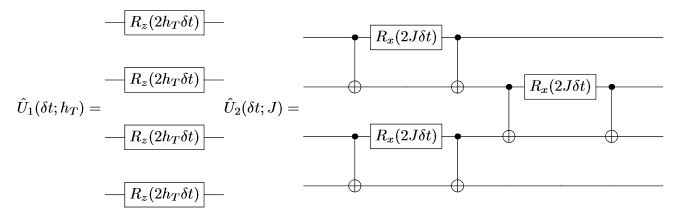
\includegraphics[width=\textwidth]{circuits2.JPG}
\caption{Terms in the Trotter operator, $\hat{U}_1(\delta t; h_T)$ and $\hat{U}_2(\delta t; J)$, 
where $R_x^J(\delta t) = e^{i J \delta t \hat{X}}$ and $R_z^{h_T}(\delta t) = e^{i \delta t h_T \hat{Z}}$.}
\label{fig:trotteroperators}
\end{figure*}

We study the transverse Ising model (TIM) with open boundary conditions (OBC) which  has the system Hamiltonian 
\be
H_{\text{OBC}}=-J\sum_{i=1}^{N_s-1} \hat{X}_i \hat{X}_{i+1} - h_T \sum_{i=1}^{N_s} \hat{Z}_i. \label{eq:H_OBC}
\ee
\LK{If we never use PBC, do we need the OBC label?}
The operators $\hat{X}_i$ and $\hat{Z}_i$ correspond to the Pauli matrices $\hat{\sigma}^x$ and $\hat{\sigma}^z$ respectively. $N_s$ corresponds to the number of sites in the model. $J$ is the nearest neighbor (hopping) coupling and controls the movement of the spins and creation of spin pairs, while $h_T$ is the on-site energy (bare mass). In this work, we will study the case with $N_s=4$, $J=0.02$ and $h_T=1$. \LK{Bare mass is not clear in all contexts
of the TFIM}.


The system can be evolved in time using the complex exponential of the Hamiltonian:
\begin{equation}
\label{eqtimeevolveexact}
\hat{U}(t) = e^{- i t \hat{H}}.
\end{equation}
Following Refs. \cite{Lloyd1073,GustafsonIsing},
the Trotter approximation %must be used because the %nearest-neighbor coupling terms do not %commute with the onsite field strength %terms the operator in Eq. %\ref{eqtimeevolveexact}. This %approximation leads to the following %expression for the time evolution %operation 
is applied to the evolution operator 
with the explicit form:
\begin{equation}
\label{eqsuzuki}
\hat{U}(t;N) = \Big(\hat{U}_1(t / N; h_t) \hat{U}_2(t / N; J)\Big)^N + \mathcal{O}(t^2 / N)
\end{equation}
where $N$ is the number of Trotter steps to be implemented, $(\delta t=\frac{t}{N})$ is the Trotter step size
\begin{equation}
\label{eqtfieldevo}
\hat{U}_1(\delta t; h_t) = e^{-i h_T \delta t \sum_{i = 1}^{4} \hat{Z}_i },
\end{equation}
and
\begin{equation}
\label{eqhoppingevo}
\hat{U}_2(\delta t; J) = e^{-i J \delta t \sum_{i = 1}^{3} \hat{X}_i \hat{X}_{i+1}}
\end{equation}
\LK{are the exponentials of the 1- and 2-body operators in the Hamiltonian.}
The operators defined in Eqs. \ref{eqtfieldevo}  and \ref{eqhoppingevo} can be expressed as a combination of the two quantum circuits shown in Fig. \ref{fig:trotteroperators}.




